%!TEX program = lualatex

\PassOptionsToPackage{french}{babel}
\PassOptionsToPackage{french}{translator}
\PassOptionsToPackage{table,svgnames}{xcolor}
\documentclass[aspectratio=169,11pt]{beamer}

%----------------------------------------
% Packages
%----------------------------------------
\usepackage{etoolbox}
\usepackage{ifxetex}
\usepackage{ifluatex}
\usepackage[T1]{fontenc}
\ifboolexpr{bool{xetex} or bool{luatex}}{%
	\usepackage{fontspec}
}{%
	\usepackage[utf8]{inputenc}
}
\usepackage{babel}
\usepackage{translator}
\usepackage{lmodern}
\usepackage{hyperref}
\usepackage{xcolor}
\usepackage{listings}
\usepackage{amsmath}
\usepackage{amssymb}
\usepackage{mathrsfs}
\usepackage{dsfont}
\usepackage{braket}
\usepackage{array}
\usepackage{tabularx}
\usepackage{multirow}
\usepackage{booktabs}
\usepackage[justification=centering]{caption}
\usepackage{float}
\usepackage[mode=tex]{standalone}
\usepackage{pgf}
\usepackage{pgfplots}
\pgfplotsset{compat=newest}
\usepackage{tikz}
\usepackage{tikzpeople}
\usepackage[backend=bibtex,bibstyle=ieee,citestyle=numeric-comp]{biblatex}

%----------------------------------------
% Theme
%----------------------------------------

\usetheme[nofirafonts,numbering=progressbar]{focus}
% \usetheme[numbering=fullbar]{focus}
% \usetheme[numbering=none]{focus}
% \definecolor{main}{RGB}{92, 138, 168}
% \definecolor{background}{RGB}{240, 247, 255}

% remove navigation symbols.
\beamertemplatenavigationsymbolsempty{}

%\setbeamercovered{transparent}

%----------------------------------------
% Informations
%----------------------------------------

\title{Set Cover Problem}
\subtitle{}
\author{Benoît Cortier\\Maxime Pinard}
\institute[UQAC]{Université du Québec à Chicoutimi\\555 Boulevard de l'Université, Chicoutimi, QC G7H 2B1}
\date[18/04/2019]{18 Avril 2019}

%\keywords{}
\subject{Set Cover Problem}
%\logo{\includegraphics[width=0.12\textwidth]{logos/UQAC}}

%----------------------------------------
% Bibliography
%----------------------------------------

\bibliography{../references}
\nocite{*}

%----------------------------------------
% Figures
%----------------------------------------

% Common file
\usetikzlibrary{shapes}
\usetikzlibrary{arrows.meta}
\usetikzlibrary{calc}
\usetikzlibrary{positioning}
\usetikzlibrary{angles}
\usetikzlibrary{quotes}
\usetikzlibrary{decorations}

\definecolor{bg_color}{RGB}{250,250,229}
\definecolor{Cblue}{RGB}{38,75,150}
\definecolor{Cgreen}{RGB}{39,179,118}
\definecolor{Cdarkgreen}{RGB}{0,111,60}
\definecolor{Corange}{RGB}{249,167,62}
\definecolor{Cred}{RGB}{191,33,47}

\colorlet{good}{green!90!black}
\colorlet{average}{Corange}
\colorlet{bad}{Cred}


% Figures folder
\graphicspath{{../figures/}}

%----------------------------------------
% Tables
%----------------------------------------

% Common file
\newcolumntype{L}[1]{>{\raggedright\let\newline\\\arraybackslash\hspace{0pt}}m{#1}}
\newcolumntype{C}[1]{>{\centering\let\newline\\\arraybackslash\hspace{0pt}}m{#1}}
\newcolumntype{R}[1]{>{\raggedleft\let\newline\\\arraybackslash\hspace{0pt}}m{#1}}
\newcolumntype{Y}{>{\centering\arraybackslash}X}


%----------------------------------------
% Plots
%----------------------------------------

\pgfplotsset{
	table/search path={../plots},
}

%----------------------------------------
% Document
%----------------------------------------
\begin{document}
	\begin{frame}
		\titlepage
	\end{frame}
	% \begin{frame}{Sommaire}
	% 	\tableofcontents
	% \end{frame}

	%% définition du problème

	\begin{frame}
		\frametitle{Définition du « Set Cover Problem » (SCP)}
		\begin{itemize}
			\item l'un des 21 problèmes NP-complets de \citeauthor{Karp1972}~\cite{Karp1972}.
			\item NP-complet au sens fort~\cite{garey2002computers}.
			\item Soit l'ensemble univers \(U = \{u_1, u_2, u_3, \dots, u_m\}\) et une famille \(S = \{s_1, s_2, \dots, s_n\}\) de sous-ensembles de \(U\).
			\item[\(\rightarrow\)] Trouver une sous-famille de \(S\) la plus petite possible permettant de couvrir chaque élément de \(U\) au moins une fois.
			\item \(e\) est couvert par un sous-ensemble \(A\) si \(e \in A\).
			\vfill
			\item En associant un coût positif \(c_i\) à chaque sous-ensemble, on obtient le problème de couverture d'ensemble pondéré ou \emph{Weighted Set Covering Problem} (WSCP)~\cite{Vazirani2003}
		\end{itemize}
	\end{frame}

	%% exemple minimal

	\begin{frame}
		\frametitle{Exemple minimal}
		\centering
		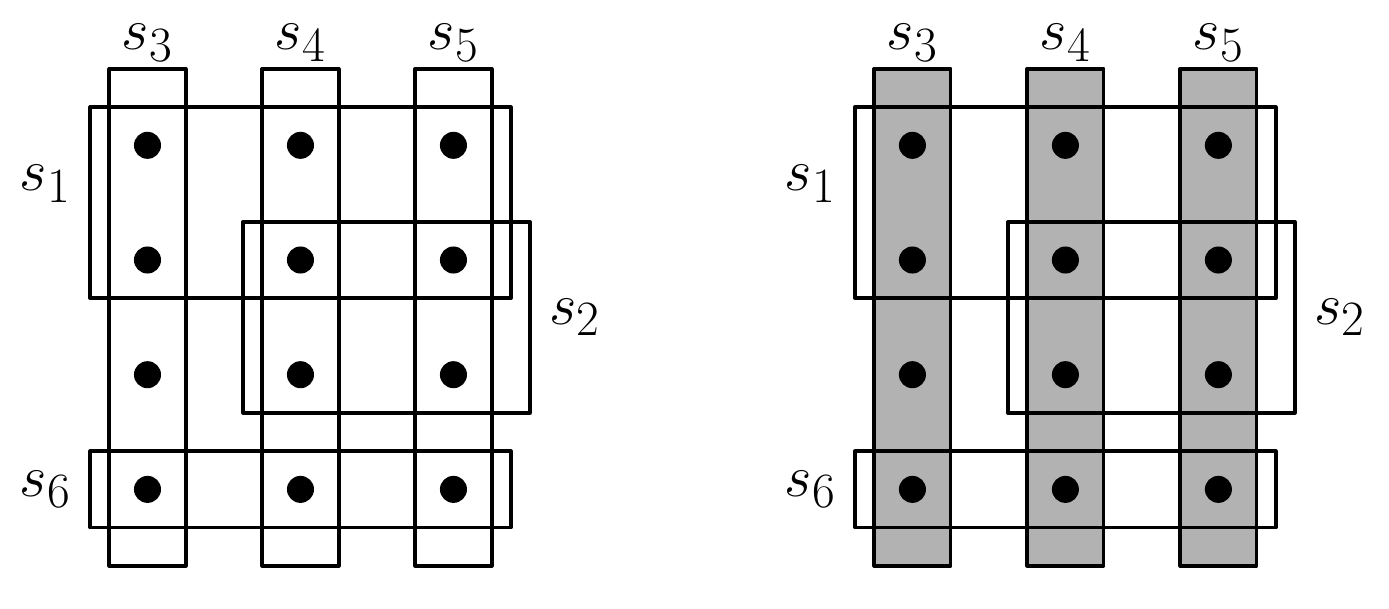
\includegraphics[width=0.75\linewidth]{scp_example}%
	\end{frame}

	%% complexité NP-complétude

	\begin{frame}
		\frametitle{Réductions de Karp}
		\centering
		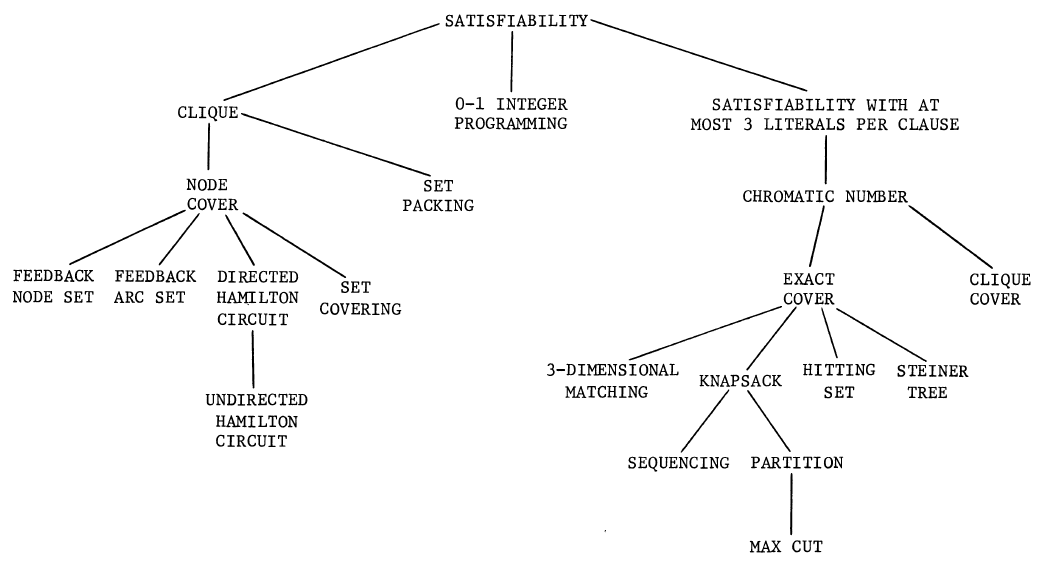
\includegraphics[width=\linewidth]{karp_reduction_tree}%
	\end{frame}

	%% état de l'art

	\begin{frame}
		\centering TODO
	\end{frame}

	%% représentation du problème

	\begin{frame}
		\centering TODO
	\end{frame}

	%% méthodes exactes

	\begin{frame}
		\centering TODO
	\end{frame}

	%% méthodes approchées

	\begin{frame}
		\centering TODO
	\end{frame}

	%% OR-library

	\begin{frame}
		\centering TODO
	\end{frame}

	%% comparaison avec les méthodes approchées

	\begin{frame}
		\centering TODO
	\end{frame}

	\begin{frame}
		\frametitle{Exemple: figure}
		\centering
		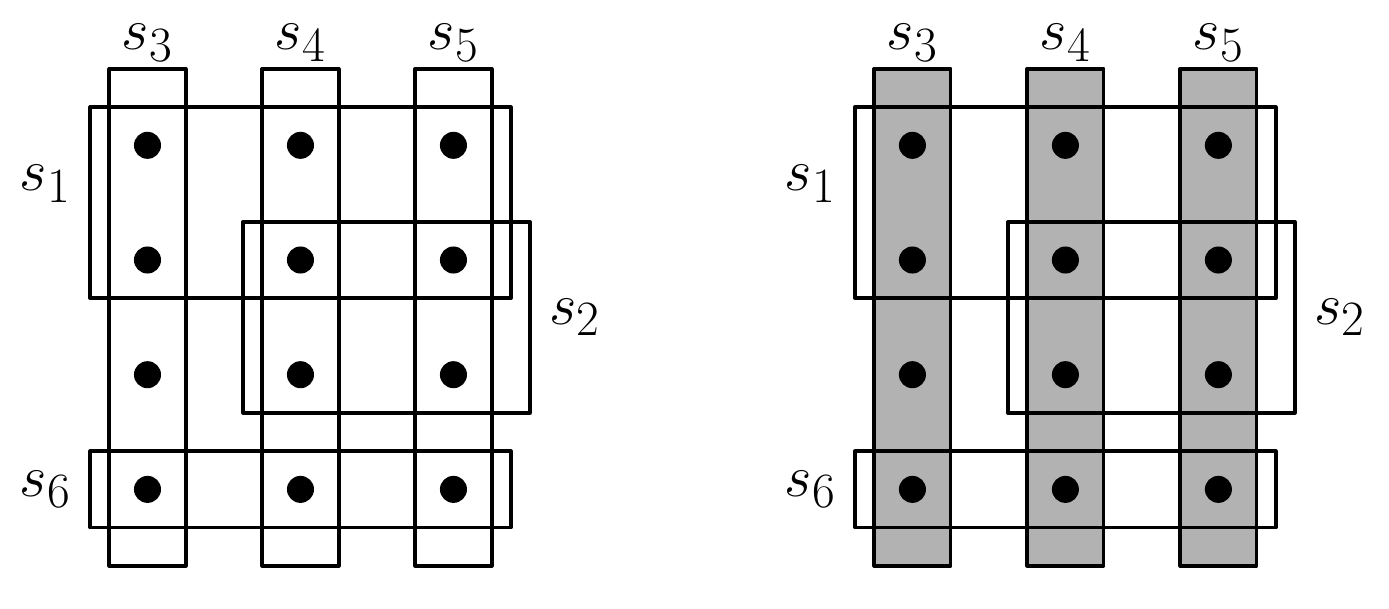
\includegraphics[width=0.75\linewidth]{scp_example}%
	\end{frame}
	\begin{frame}
		\frametitle{Exemple: table}
		{
			\centering
			\footnotesize
			%!TEX root = ../set_cover_problem.tex
\begin{tabular}{*{5}{C{65pt}}}
	\toprule
	Groupe d'instances & Nombre de lignes (\(m\)) [points] & Nombre de colonnes (\(n\)) [sous-ensembles] & densité (\%) & Nombre d'instances du groupe\\
	\midrule
	4 & 200 & 1000 & 2 & 10\\
	5 & 200 & 2000 & 2 & 10\\
	6 & 200 & 1000 & 5 & 5\\
	A & 300 & 3000 & 2 & 5\\
	B & 300 & 3000 & 5 & 5\\
	C & 400 & 4000 & 2 & 5\\
	D & 400 & 4000 & 5 & 5\\
	E & 500 & 5000 & 10 & 5\\
	F & 500 & 5000 & 20 & 5\\
	G & 1000 & 10000 & 2 & 5\\
	H & 1000 & 10000 & 5 & 5\\
	\bottomrule
\end{tabular}
		}
	\end{frame}
	\begin{frame}
		\frametitle{Exemple: plot}
		\centering
		\begin{tikzpicture}
	\begin{axis}[
		width=\linewidth,
		height=0.5\linewidth,
		xlabel={taille du bitset (nombre de bits)},
		ylabel={RAM utilisée (Go)},
		xmin=0, xmax=40,
		ymin=0, ymax=9,
		legend style={
			cells={
				anchor=west
			},
			legend pos=north west,
		},
	]
		\addplot[smooth,color=blue,mark=square*] table{g1_ram.data};
		\addlegendentry{G1: ram expensive generator}
		\addplot[smooth,color=red,mark=*] table{g2_ram.data};
		\addlegendentry{G2: cpu expensive generator}
		\addplot[smooth,color=cyan,mark=triangle*] table{g3_ram.data};
		\addlegendentry{G3: counter generator}
	\end{axis}
\end{tikzpicture}%%
	\end{frame}
	\section*{Questions?}
		\begin{frame}[focus]
			Questions?
		\end{frame}
	\appendix
		\begin{frame}[t,allowframebreaks]
			\frametitle{Références}
			\printbibliography[heading=bibintoc]{}
		\end{frame}
\end{document}
